\documentclass[tikz,border=5pt]{standalone}
\usepackage{amsmath}
\usetikzlibrary{arrows.meta, decorations.pathmorphing, calc}

\begin{document}
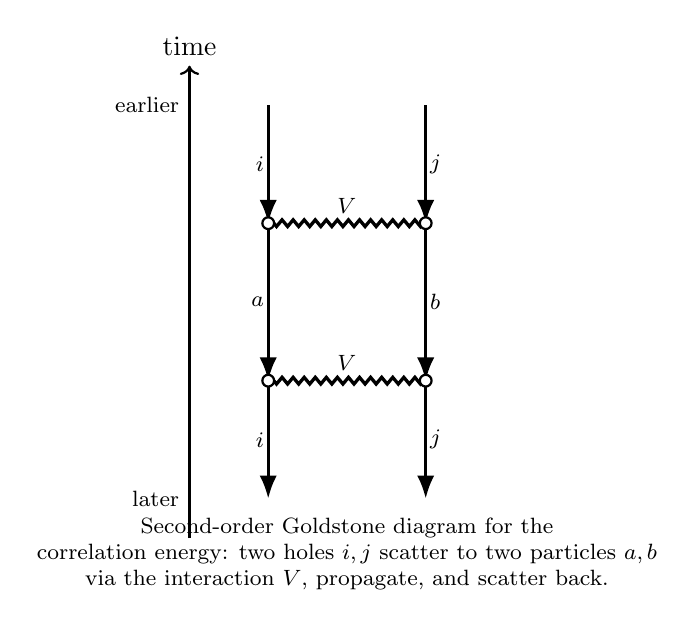
\begin{tikzpicture}[
   thick,
=Latex,
   hole/.style={-Latex, very thick},        % hole lines (downward arrows)
   part/.style={Latex-, very thick},        % particle lines (upward arrows)
   vint/.style={decorate, decoration={zigzag,segment length=4pt,amplitude=1.2pt}, very thick},
   vertex/.style={draw, fill=white, circle, inner sep=1.5pt},
   labelstyle/.style={font=\footnotesize, fill=white, inner sep=1pt},
   baseline={(current bounding box.center)}
]

% coordinate helpers:
% We'll draw two interaction vertices at y=0 and y=2.
% Holes (incoming, going downward in time) start below y=0.
% Particles (excited, propagating above Fermi surface) go above y=2.

% --- positions of vertices
\coordinate (V1L) at (-1,0);   % left leg of lower vertex
\coordinate (V1R) at ( 1,0);   % right leg of lower vertex
\coordinate (V2L) at (-1,2);   % left leg of upper vertex
\coordinate (V2R) at ( 1,2);   % right leg of upper vertex

% --- external hole lines (i and j) entering bottom vertex from below
\coordinate (i_in) at (-1,-1.5);
\coordinate (j_in) at ( 1,-1.5);

% --- external hole lines going out of top vertex upward?
% In Goldstone time-ordering, holes actually propagate downward
% (i.e. you read from top to bottom in energy-time MBPT convention).
% We'll instead label outgoing as same i,j for clarity.
\coordinate (i_out) at (-1,3.5);
\coordinate (j_out) at ( 1,3.5);

% --- intermediate particle lines a,b between the two vertices
% We'll draw a and b going upward between V1 and V2,
% which represent particle propagation above the Fermi surface.
% Then connect back down at the second vertex.

% Draw HOLE LINES:
% In standard Goldstone notation: hole lines point downward in time.
% We'll annotate arrows downward. For pedagogy we'll still show
% external "legs" continuing, but emphasize direction with arrows.

% hole i line: from i_in up to V1L (arrow downward)
\draw[hole] (V1L) -- (i_in)
   node[midway, anchor=east, labelstyle] {$i$};

% then from V2L up to i_out (arrow downward, so reverse arrow direction when drawing upward path)
\draw[hole] (i_out) -- (V2L)
   node[midway, anchor=east, labelstyle] {$i$};

% connect V1L to V2L (this is actually a particle line up, not hole; we'll handle below)
% For cleanliness we'll not double-draw; we'll instead draw internal lines separately.

% hole j line: from j_in up to V1R
\draw[hole] (V1R) -- (j_in)
   node[midway, anchor=west, labelstyle] {$j$};

% and from V2R up to j_out
\draw[hole] (j_out) -- (V2R)
   node[midway, anchor=west, labelstyle] {$j$};

% --- PARTICLE LINES a,b between vertices:
% After first interaction, two particles a,b propagate upward and meet again.

% We'll route them with slight horizontal bending to avoid overlap.

\coordinate (a_mid1) at (-1,0);   % created at lower left vertex
\coordinate (a_mid2) at (-1,2);   % annihilated at upper left vertex

\coordinate (b_mid1) at ( 1,0);   % created at lower right vertex
\coordinate (b_mid2) at ( 1,2);   % annihilated at upper right vertex

% particle a line (arrow upward = particle propagation)
\draw[part] (a_mid1) .. controls (-1,1) and (-1,1) .. (a_mid2)
   node[midway, anchor=east, labelstyle] {$a$};

% particle b line (arrow upward)
\draw[part] (b_mid1) .. controls ( 1,1) and ( 1,1) .. (b_mid2)
   node[midway, anchor=west, labelstyle] {$b$};

% --- Interaction lines (two-body interaction) between the two fermion lines:
% We'll draw wavy / zigzag line connecting the two vertices at each time slice.
% First interaction at bottom vertex between (i,j)->(a,b)
% Second interaction at top vertex between (a,b)->(i,j)

\draw[vint] (V1L) -- (V1R)
   node[midway, above=2pt, labelstyle] {$V$};

\draw[vint] (V2L) -- (V2R)
   node[midway, above=2pt, labelstyle] {$V$};

% --- Draw the actual vertices as dots:
\node[vertex] at (V1L) {};
\node[vertex] at (V1R) {};
\node[vertex] at (V2L) {};
\node[vertex] at (V2R) {};

% --- Add time arrow
\draw[->, thick] (-2,-2) -- (-2,4) node[anchor=south] {time};

\node[anchor=east, font=\footnotesize] at (-2,3.5) {earlier};
\node[anchor=east, font=\footnotesize] at (-2,-1.5) {later};

% --- Caption box under diagram
\node[align=center, font=\footnotesize] at (0,-2.2)
{Second-order Goldstone diagram for the\\
correlation energy:
two holes $i,j$ scatter to two particles $a,b$\\
via the interaction $V$, propagate, and scatter back.};

\end{tikzpicture}
\end{document}